%%%%%%%%%%%%%%%%%%%%%%%%%%%%%%%%%%%%%%%%%%%%%%%%%%%%%%%%%%%%%%%%%%%%%%%%%%%%%%%%%%
\begin{frame}[fragile]\frametitle{}
\begin{center}
{\Large Introduction to Graph RAG}
\end{center}
\end{frame}

% %%%%%%%%%%%%%%%%%%%%%%%%%%%%%%%%%%%%%%%%%%%%%%%%%%%%%%%%%%%
% \begin{frame}[fragile]\frametitle{Challenges with LLMs}
    % \begin{itemize}
        % \item Learns random sentences from random people
        % \item Talks like a person but doesn't really understand what it's saying
        % \item Occasionally speaks absolute non sense
        % \item Sensitive to question phrasing
        % \item Limited to public ``knowledge''
    % \end{itemize}
	
	% {\tiny (Ref: The GenAI Stack - Andreas Kollegger - Neo4j)}
	
% \end{frame}

% %%%%%%%%%%%%%%%%%%%%%%%%%%%%%%%%%%%%%%%%%%%%%%%%%%%%%%%%%%%
% \begin{frame}[fragile]\frametitle{Thematic RAG Classification}

	% \begin{center}
	% 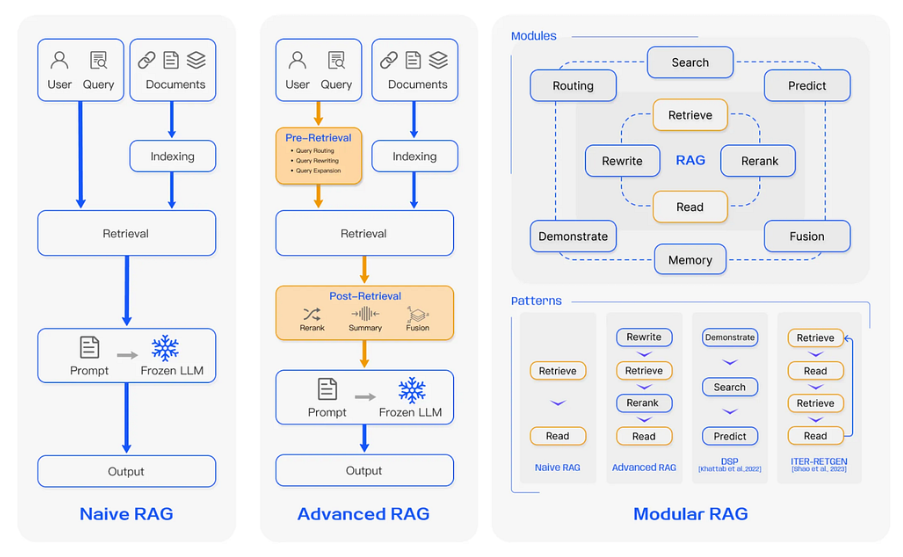
\includegraphics[width=\linewidth,keepaspectratio]{graphrag14}
	% \end{center}
	
		% {\tiny (Ref: https://graphrag.com/concepts/intro-to-graphrag/))}

	
% \end{frame}

% %%%%%%%%%%%%%%%%%%%%%%%%%%%%%%%%%%%%%%%%%%%%%%%%%%%%%%%%%%%
% \begin{frame}[fragile]\frametitle{The phases of an advanced RAG system}
    % \begin{itemize}
        % \item Pre-retrieval-Query rewriting, query entity extraction, query expansion, etc.
        % \item Retrieval of relevant context
        % \item Post-retrieval: Reranking, pruning, etc.
        % \item Answer generation
    % \end{itemize}
	
		% {\tiny (Ref: https://graphrag.com/concepts/intro-to-graphrag/))}
	
% \end{frame}


%%%%%%%%%%%%%%%%%%%%%%%%%%%%%%%%%%%%%%%%%%%%%%%%%%%%%%%%%%%
\begin{frame}[fragile]\frametitle{Why Graph RAG?}
    \begin{itemize}
        \item Language models struggle with factual accuracy and real-world knowledge.
        \item Retrieval-Augmented Generation (RAG) improves accuracy using external text data.
        \item Traditional RAG has limitations in context understanding and scalability.
        \item GraphRAG leverages knowledge graphs for better retrieval and response generation.
    \end{itemize}
\end{frame}

%%%%%%%%%%%%%%%%%%%%%%%%%%%%%%%%%%%%%%%%%%%%%%%%%%%%%%%%%%%
\begin{frame}[fragile]\frametitle{Overview of Traditional RAG}
	
	\begin{center}
	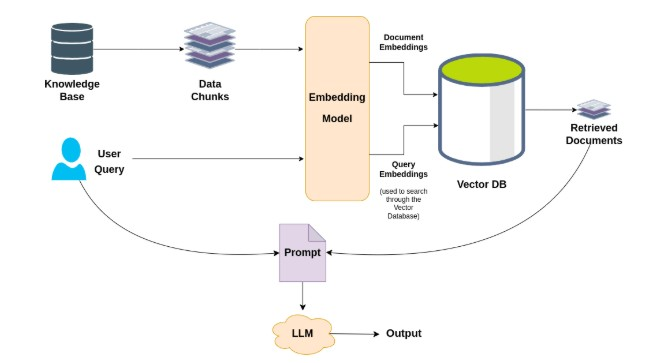
\includegraphics[width=\linewidth,keepaspectratio]{graphrag16}
	
	{\tiny (Ref: GraphRAG: The Practical Guide for Cost-Effective Document Analysis with Knowledge Graphs -Jaykumaran)}
	\end{center}	
\end{frame}

%%%%%%%%%%%%%%%%%%%%%%%%%%%%%%%%%%%%%%%%%%%%%%%%%%%%%%%%%%%
\begin{frame}[fragile]\frametitle{Limitations of Traditional RAG}
    \begin{itemize}
		\item Answer has to be in the chunk fully, cannot be across the chunks.
		\item Cannot have multiple chunks compose the final answer.
        \item Documents are treated as isolated entities.
        \item Lacks deep semantic understanding as multi-hop answers
        \item Slower retrieval with increasing data volume.
        \item Lacks global context over the entire data corpus.
        \item Inefficient for complex reasoning across multiple documents.
        \item Hard to trace the source of retrieved information.
    \end{itemize}
\end{frame}

%%%%%%%%%%%%%%%%%%%%%%%%%%%%%%%%%%%%%%%%%%%%%%%%%%%%%%%%%%%
\begin{frame}[fragile]\frametitle{What is GraphRAG?}

    \begin{block}
    RAG on Graph: combines traditional RAG techniques with graph-based knowledge representations to leverage structural relationships between entities.
    \end{block}
\end{frame}


%%%%%%%%%%%%%%%%%%%%%%%%%%%%%%%%%%%%%%%%%%%%%%%%%%%%%%%%%%%
\begin{frame}[fragile]\frametitle{Vector RAG vs GraphRAG}

	
	\begin{center}
	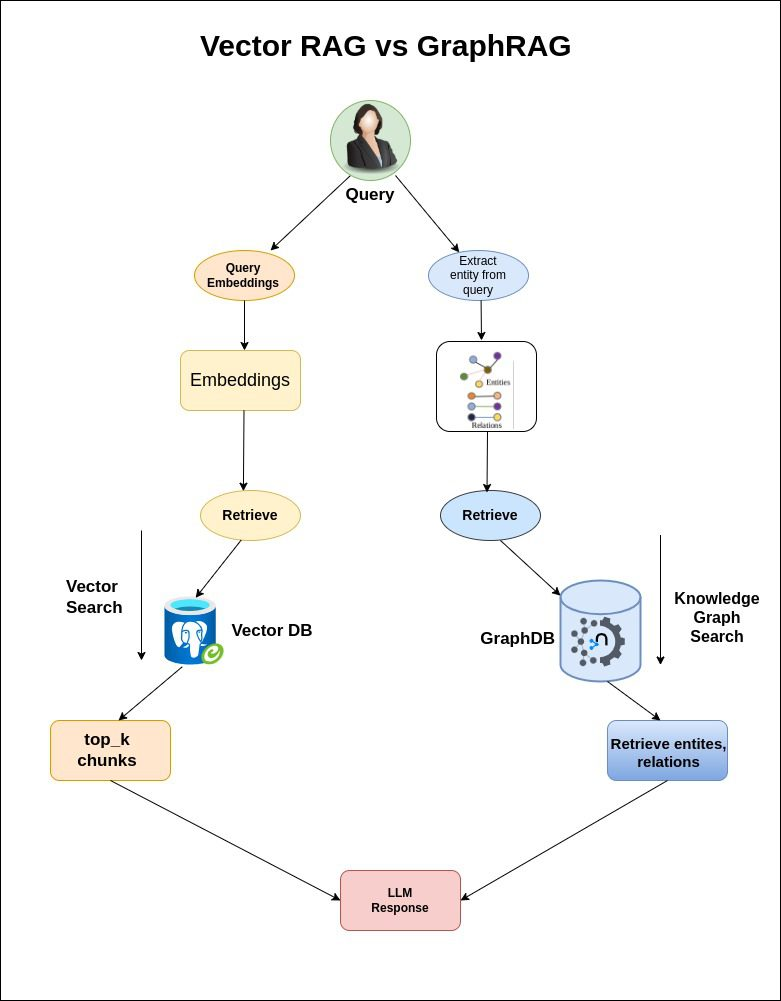
\includegraphics[width=0.5\linewidth,keepaspectratio]{graphrag17}
	
	{\tiny (Ref: GraphRAG: The Practical Guide for Cost-Effective Document Analysis with Knowledge Graphs -Jaykumaran)}
	\end{center}	
\end{frame}

%%%%%%%%%%%%%%%%%%%%%%%%%%%%%%%%%%%%%%%%%%%%%%%%%%%%%%%%%%%
\begin{frame}[fragile]\frametitle{Traditional RAG vs GraphRAG}
    \begin{table}[]
        \centering
        \begin{tabular}{|l|l|l|}
            \hline
            \textbf{Feature} & \textbf{Traditional RAG} & \textbf{GraphRAG} \\
            \hline
            Data Representation & Flat Vectors & Knowledge Graph \\
            \hline
            Query Scope & Local context & Global Reasoning \\
            \hline
            Scalability & Low & High \\
            \hline
            Citation Transparency & Low & High (Traceable sources) \\
            \hline
            Response Coherence & Fragmented & Relevant and Context-Rich \\
            \hline
        \end{tabular}
    \end{table}
\end{frame}

%%%%%%%%%%%%%%%%%%%%%%%%%%%%%%%%%%%%%%%%%%%%%%%%%%%%%%%%%%%
\begin{frame}[fragile]\frametitle{How GraphRAG Solves the Problem}
    \begin{itemize}
        \item GraphRAG combines graph structures with vector search.
        \item Traverses multi-hop connections to infer relationships.
        \item Offers more reliable responses than vector-only RAG.
    \end{itemize}

\textit{Graph-based RAG helps agentic AI make human-like decisions.} 
– May Habib, CEO of Writer.com
\end{frame}




%%%%%%%%%%%%%%%%%%%%%%%%%%%%%%%%%%%%%%%%%%%%%%%%%%%%%%%%%%%
\begin{frame}[fragile]\frametitle{Different Approaches}


	\begin{itemize}
	\item English Query is converted to GraphQL or Cypher query then calls GraphDB to fetch the context/answers. Uses few-shots or specialized parsers or fine-tuned LLMs for the conversion (Neo4j way). 
	\item Knowledge Graph is indexed, then English query then sent to index (which fetches, relevant triplets, also node's data), , KG may be created by LLM Graph Transformer and put in NetworkX object, you can populate this externally as well. (Langchain/Llamaindex way)
	\item From documents, populates the Knowledge Graph first, indexes it, then brings the relevant context from the index (Microsoft way)
	\item Contextual Subgraph/Path-based Retrieval Approach: Extracts reasoning paths or connected subgraphs for the input query (mostly academic research)
	\end{itemize}

\end{frame}


%%%%%%%%%%%%%%%%%%%%%%%%%%%%%%%%%%%%%%%%%%%%%%%%%%%%%%%%%%%
\begin{frame}[fragile]\frametitle{Example: Medical Query Challenge}
    \begin{itemize}
        \item Query: How does Medication A in Patient Record 1 affect Condition B in Patient Record 2?
        \item LLM needs to infer relationships across multiple records.
        \item Standard RAG struggles with such complex dependencies.
        \item Scaling this to millions of patient records is infeasible.
    \end{itemize}
	
	\begin{center}
	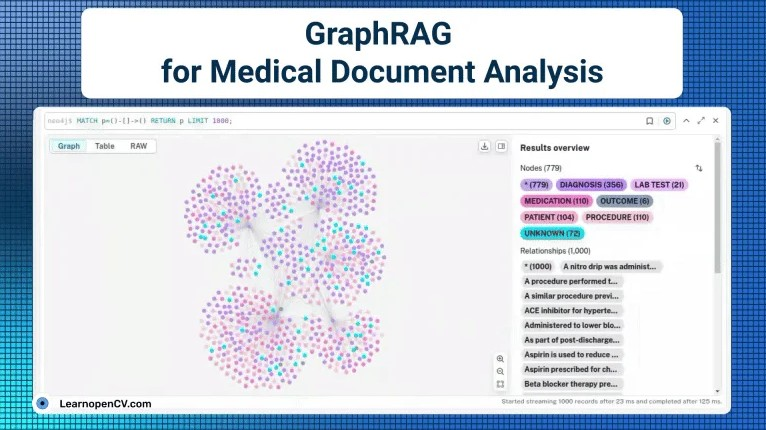
\includegraphics[width=0.8\linewidth,keepaspectratio]{graphrag15}
	
	{\tiny (Ref: GraphRAG: The Practical Guide for Cost-Effective Document Analysis with Knowledge Graphs -Jaykumaran)}
	\end{center}	
\end{frame}


% %%%%%%%%%%%%%%%%%%%%%%%%%%%%%%%%%%%%%%%%%%%%%%%%%%%%%%%%%%%
% \begin{frame}[fragile]\frametitle{How GraphRAG Works?}
    % \begin{itemize}
        % \item \textbf{Knowledge Graph Construction:} Extracts entities and relationships.
        % \item \textbf{Knowledge Graph Summarization:} Generates hierarchical summaries.
        % \item \textbf{Retrieval-Augmented Generation:} Uses local and global searches for queries.
    % \end{itemize}
% \end{frame}

% %%%%%%%%%%%%%%%%%%%%%%%%%%%%%%%%%%%%%%%%%%%%%%%%%%%%%%%%%%%
% \begin{frame}[fragile]\frametitle{Example of GraphRAG Representation}
    % \begin{lstlisting}
    % # Entities
    % Type 2 Diabetes (Condition)
    % High Blood Sugar Levels (Symptom)
    % Nerve Damage (Complication)
    % Kidney Disease (Complication)
    % Cardiovascular Problems (Complication)

    % # Relationships
    % Type 2 Diabetes -> has_symptom -> High Blood Sugar Levels
    % Type 2 Diabetes -> can_lead_to -> Nerve Damage
    % Type 2 Diabetes -> can_lead_to -> Kidney Disease
    % Type 2 Diabetes -> can_lead_to -> Cardiovascular Problems
    % \end{lstlisting}
% \end{frame}


%%%%%%%%%%%%%%%%%%%%%%%%%%%%%%%%%%%%%%%%%%%%%%%%%%%%%%%%%%%
\begin{frame}[fragile]\frametitle{Advantages of GraphRAG}
    \begin{itemize}
        \item Structured knowledge retrieval, so far less hallucinations, thus more accuracy.
        \item Context-aware and efficient retrieval.
        \item Handles complex queries effectively.
        \item Provides explainability and transparency.
    \end{itemize}
\end{frame}


%%%%%%%%%%%%%%%%%%%%%%%%%%%%%%%%%%%%%%%%%%%%%%%%%%%%%%%%%%%
\begin{frame}[fragile]\frametitle{Advantages of GraphRAG}

	\begin{center}
	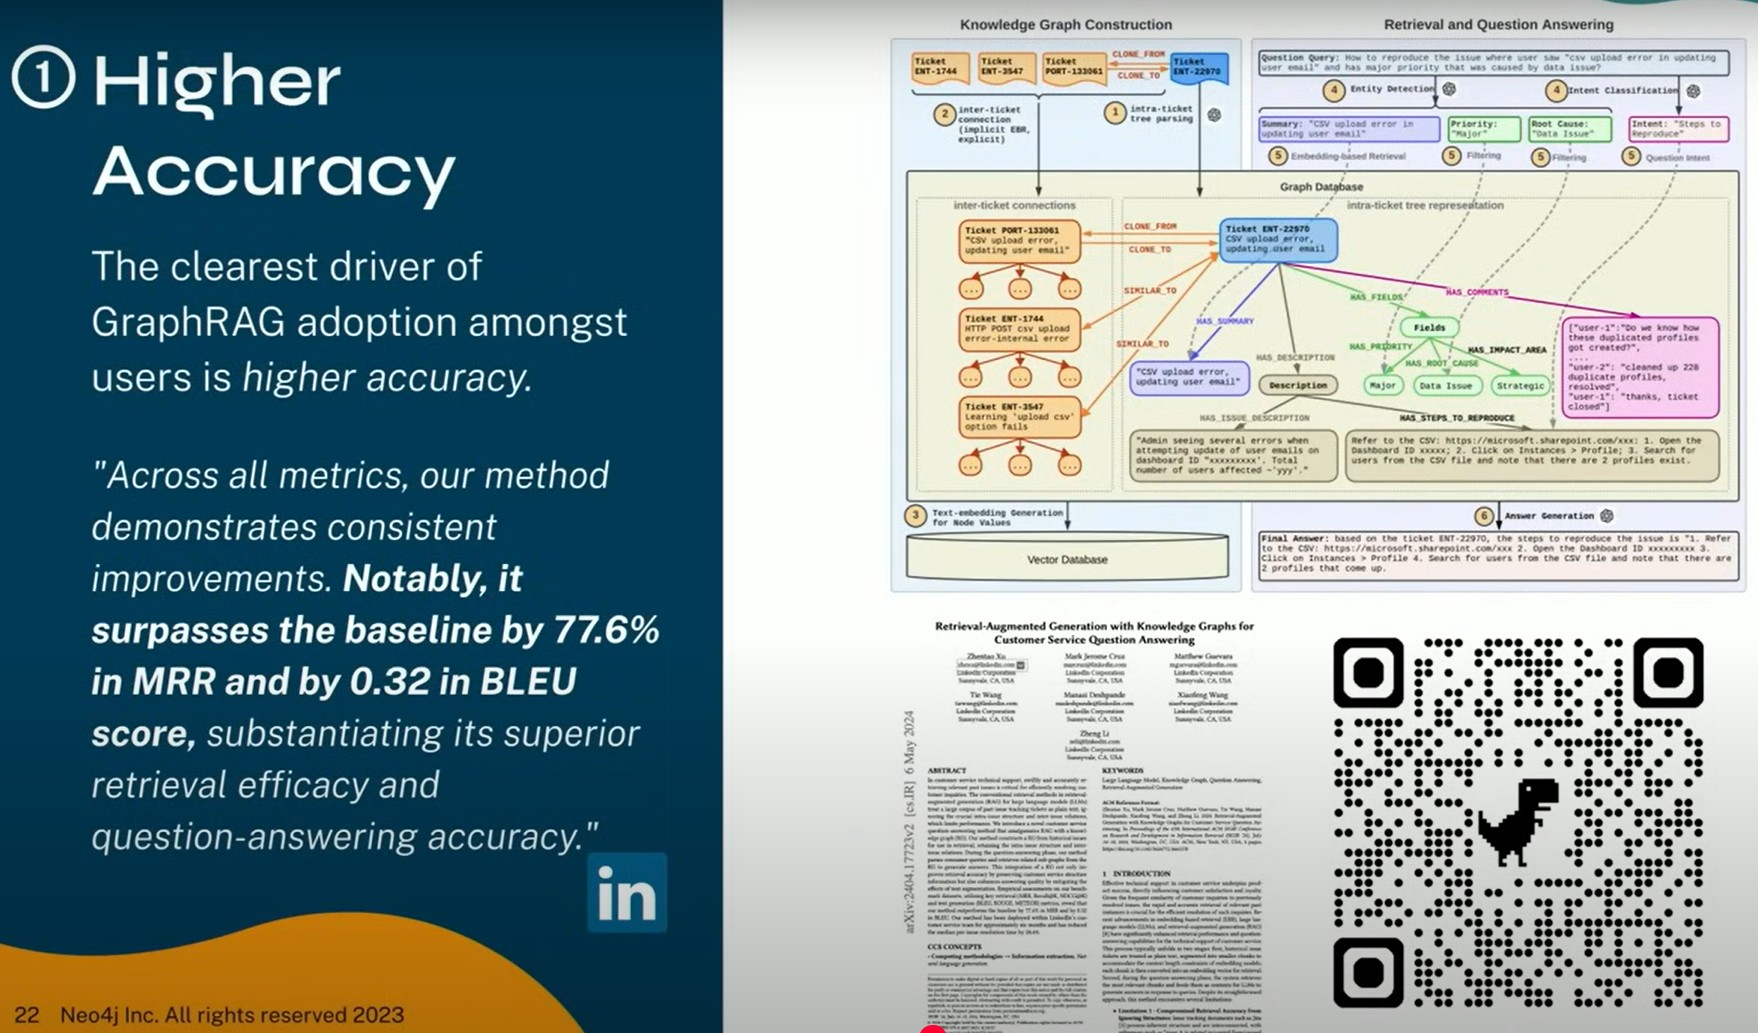
\includegraphics[width=\linewidth,keepaspectratio]{graphrag21}
	\end{center}
	
	{\tiny (Ref: GraphRAG: The Marriage of Knowledge Graphs and RAG: Emil Eifrem)}

	
\end{frame}

%%%%%%%%%%%%%%%%%%%%%%%%%%%%%%%%%%%%%%%%%%%%%%%%%%%%%%%%%%%
\begin{frame}[fragile]\frametitle{Advantages of GraphRAG}

	\begin{center}
	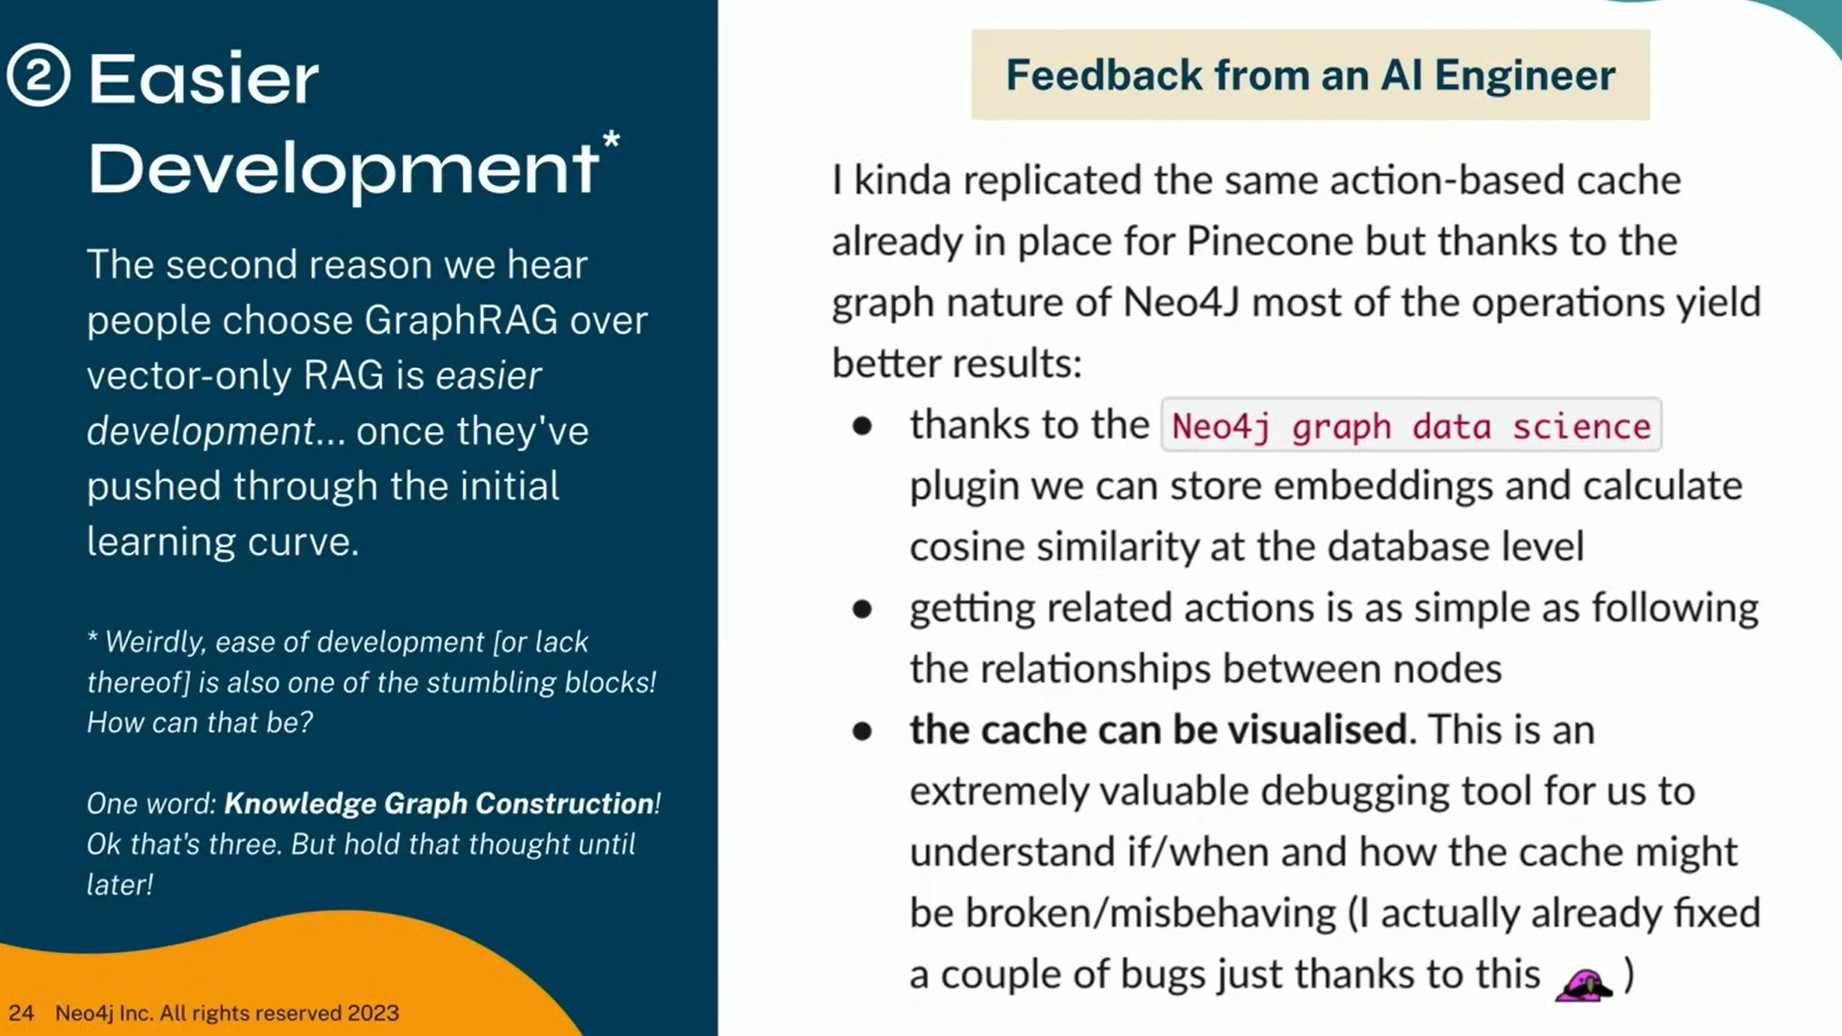
\includegraphics[width=\linewidth,keepaspectratio]{graphrag22}
	\end{center}
	
	{\tiny (Ref: GraphRAG: The Marriage of Knowledge Graphs and RAG: Emil Eifrem)}

	
\end{frame}

%%%%%%%%%%%%%%%%%%%%%%%%%%%%%%%%%%%%%%%%%%%%%%%%%%%%%%%%%%%
\begin{frame}[fragile]\frametitle{Advantages of GraphRAG}

	\begin{center}
	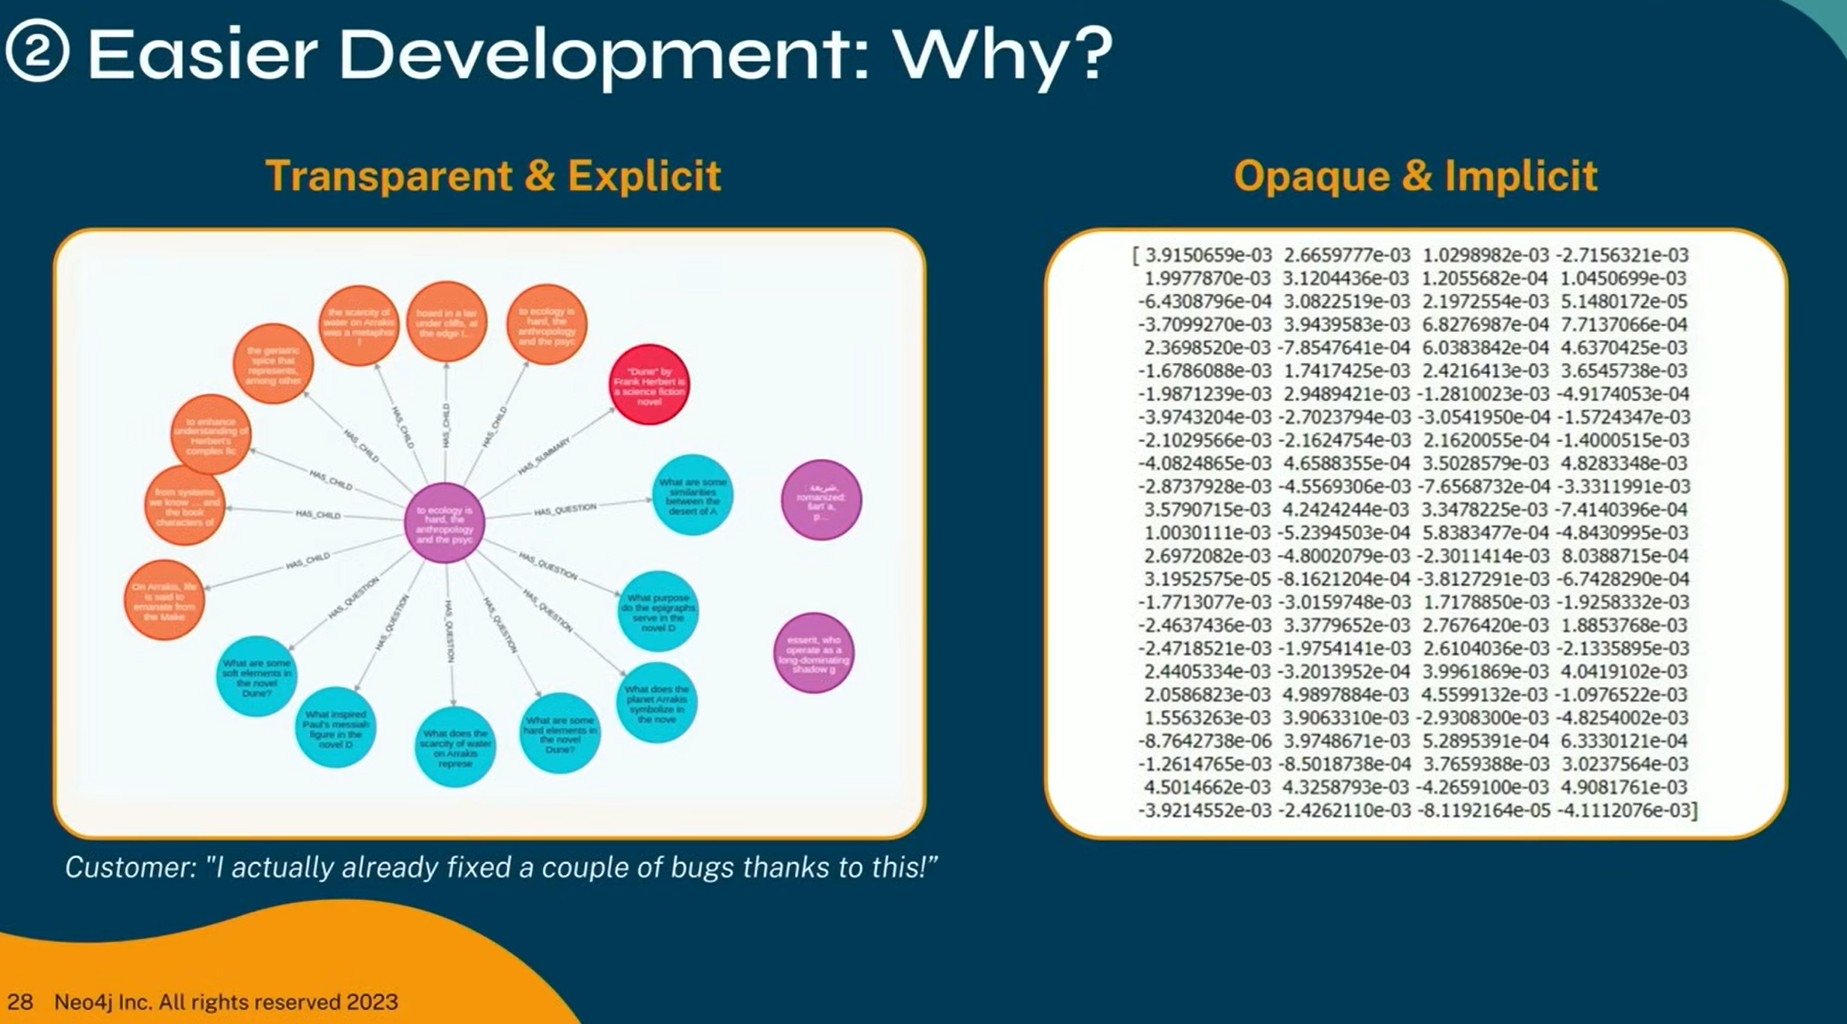
\includegraphics[width=\linewidth,keepaspectratio]{graphrag23}
	\end{center}
	
	{\tiny (Ref: GraphRAG: The Marriage of Knowledge Graphs and RAG: Emil Eifrem)}

	
\end{frame}

%%%%%%%%%%%%%%%%%%%%%%%%%%%%%%%%%%%%%%%%%%%%%%%%%%%%%%%%%%%
\begin{frame}[fragile]\frametitle{Advantages of GraphRAG}

	\begin{center}
	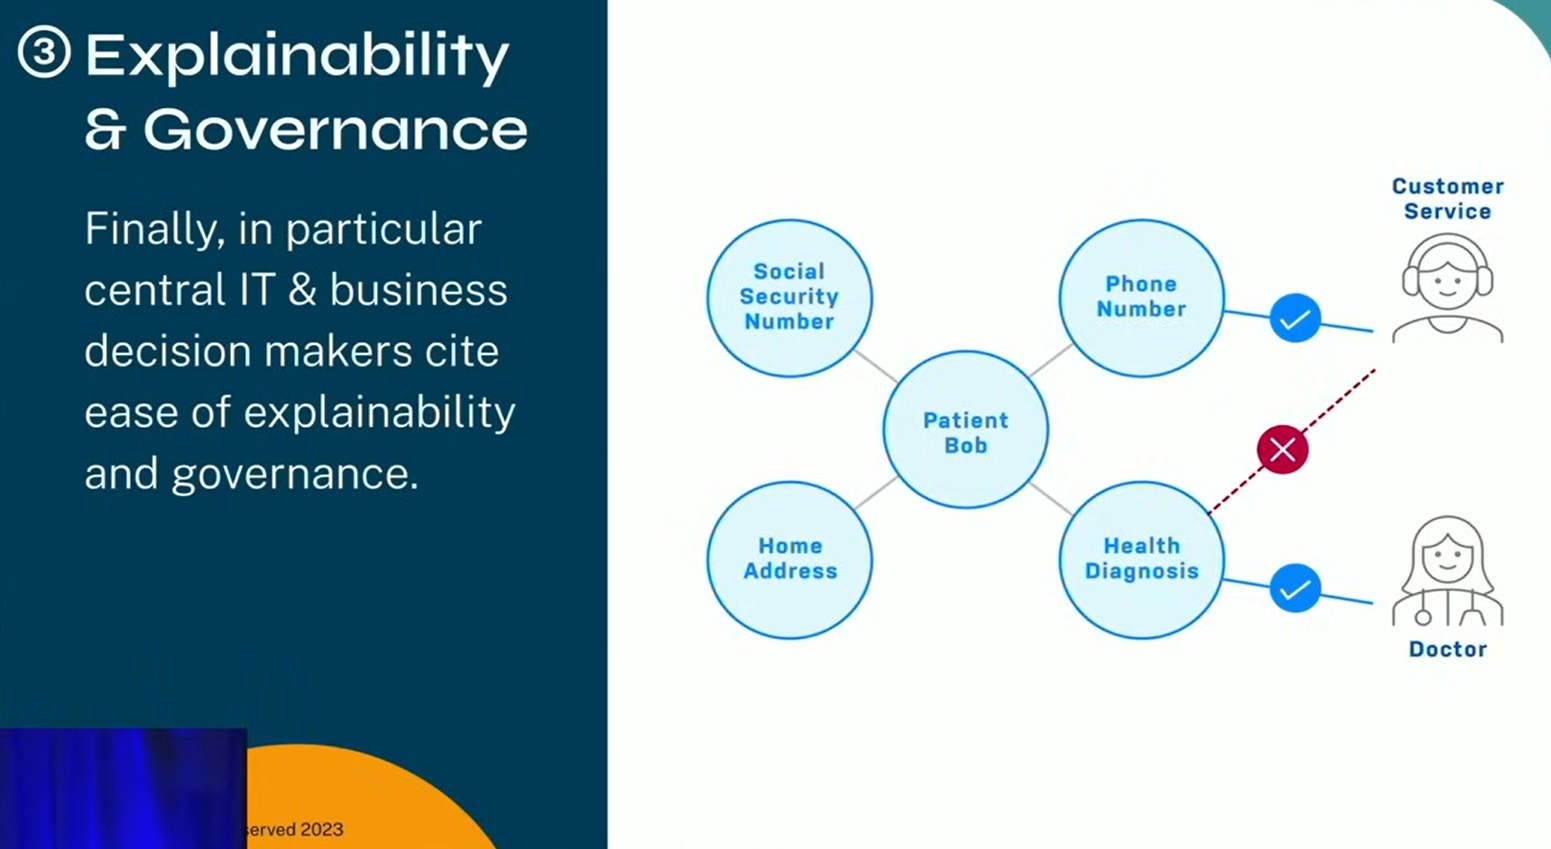
\includegraphics[width=\linewidth,keepaspectratio]{graphrag24}
	\end{center}
	
	{\tiny (Ref: GraphRAG: The Marriage of Knowledge Graphs and RAG: Emil Eifrem)}

	
\end{frame}

%%%%%%%%%%%%%%%%%%%%%%%%%%%%%%%%%%%%%%%%%%%%%%%%%%%%%%%%%%%
\begin{frame}[fragile]\frametitle{Advantages of GraphRAG}

	\begin{center}
	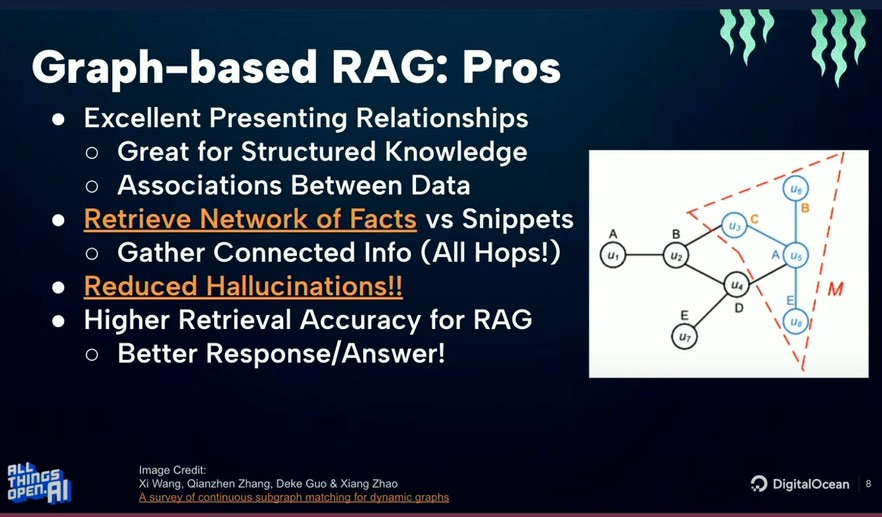
\includegraphics[width=\linewidth,keepaspectratio]{graphrag26}
	\end{center}
	
	{\tiny (Ref: Leveraging Knowledge Graphs for RAG: A Smarter Approach to Contextual AI Applications)}

	
\end{frame}


%%%%%%%%%%%%%%%%%%%%%%%%%%%%%%%%%%%%%%%%%%%%%%%%%%%%%%%%%%%
\begin{frame}[fragile]\frametitle{Challenges of GraphRAG}
    \begin{itemize}
        \item \textbf{Complex Knowledge Graph Construction:} Requires sophisticated NLP techniques.
        \item \textbf{Data Dependency:} Performance relies on input data quality.
        \item \textbf{Scalability Issues:} Large graphs require significant computational resources.
    \end{itemize}
\end{frame}

%%%%%%%%%%%%%%%%%%%%%%%%%%%%%%%%%%%%%%%%%%%%%%%%%%%%%%%%%%%
\begin{frame}[fragile]\frametitle{Challenges of GraphRAG}

	\begin{center}
	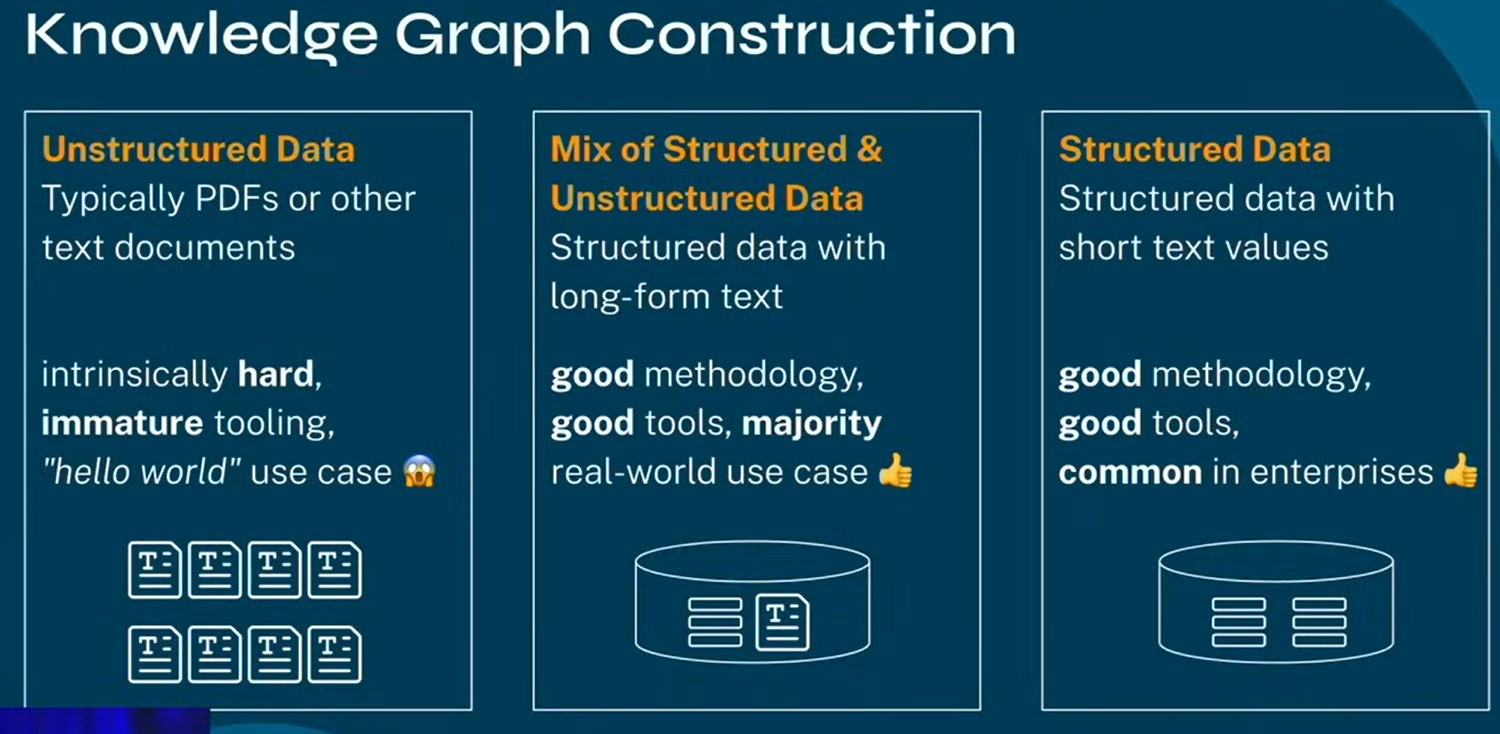
\includegraphics[width=\linewidth,keepaspectratio]{graphrag25}
	\end{center}
	
	{\tiny (Ref: GraphRAG: The Marriage of Knowledge Graphs and RAG: Emil Eifrem)}

	
\end{frame}

%%%%%%%%%%%%%%%%%%%%%%%%%%%%%%%%%%%%%%%%%%%%%%%%%%%%%%%%%%%
\begin{frame}[fragile]\frametitle{Challenges of GraphRAG}

	\begin{center}
	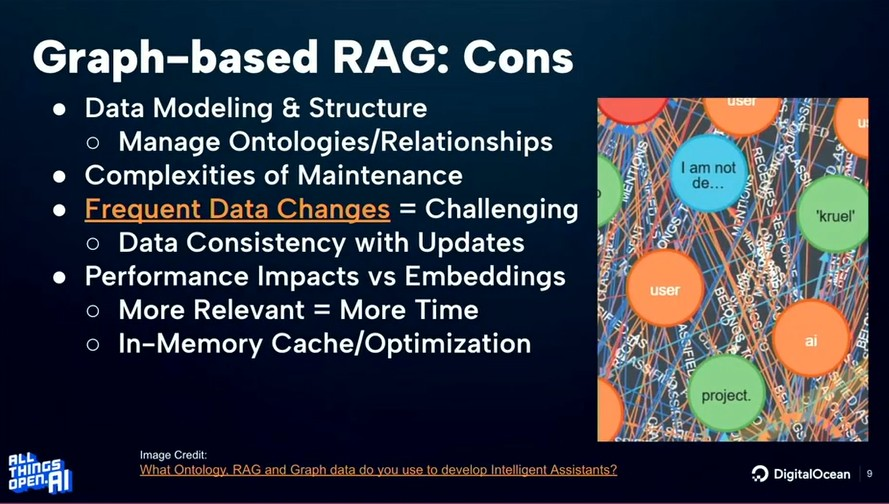
\includegraphics[width=\linewidth,keepaspectratio]{graphrag27}
	\end{center}
	
	{\tiny (Ref: Leveraging Knowledge Graphs for RAG: A Smarter Approach to Contextual AI Applications)}

	
\end{frame}


%%%%%%%%%%%%%%%%%%%%%%%%%%%%%%%%%%%%%%%%%%%%%%%%%%%%%%%%%%%
\begin{frame}[fragile]\frametitle{Applications of GraphRAG}
    \begin{itemize}
        \item \textbf{Healthcare:} Assists in diagnoses and treatment decisions.
        \item \textbf{Banking:} Detects fraudulent transactions using knowledge graphs.
        \item \textbf{Customer Service :} quickly answer customer questions from thousands of pages of policy documentation
        \item \textbf{Recommendations:} understand customer behavior and preferences better, to provide personalized services.
        \item \textbf{Supply Chain:} product recall and associated quality control checking, internal documentation search
	
    \end{itemize}

\end{frame}


%%%%%%%%%%%%%%%%%%%%%%%%%%%%%%%%%%%%%%%%%%%%%%%%%%%%%%%%%%%
\begin{frame}[fragile]\frametitle{Trend of GraphRAG Research}

	\begin{center}
	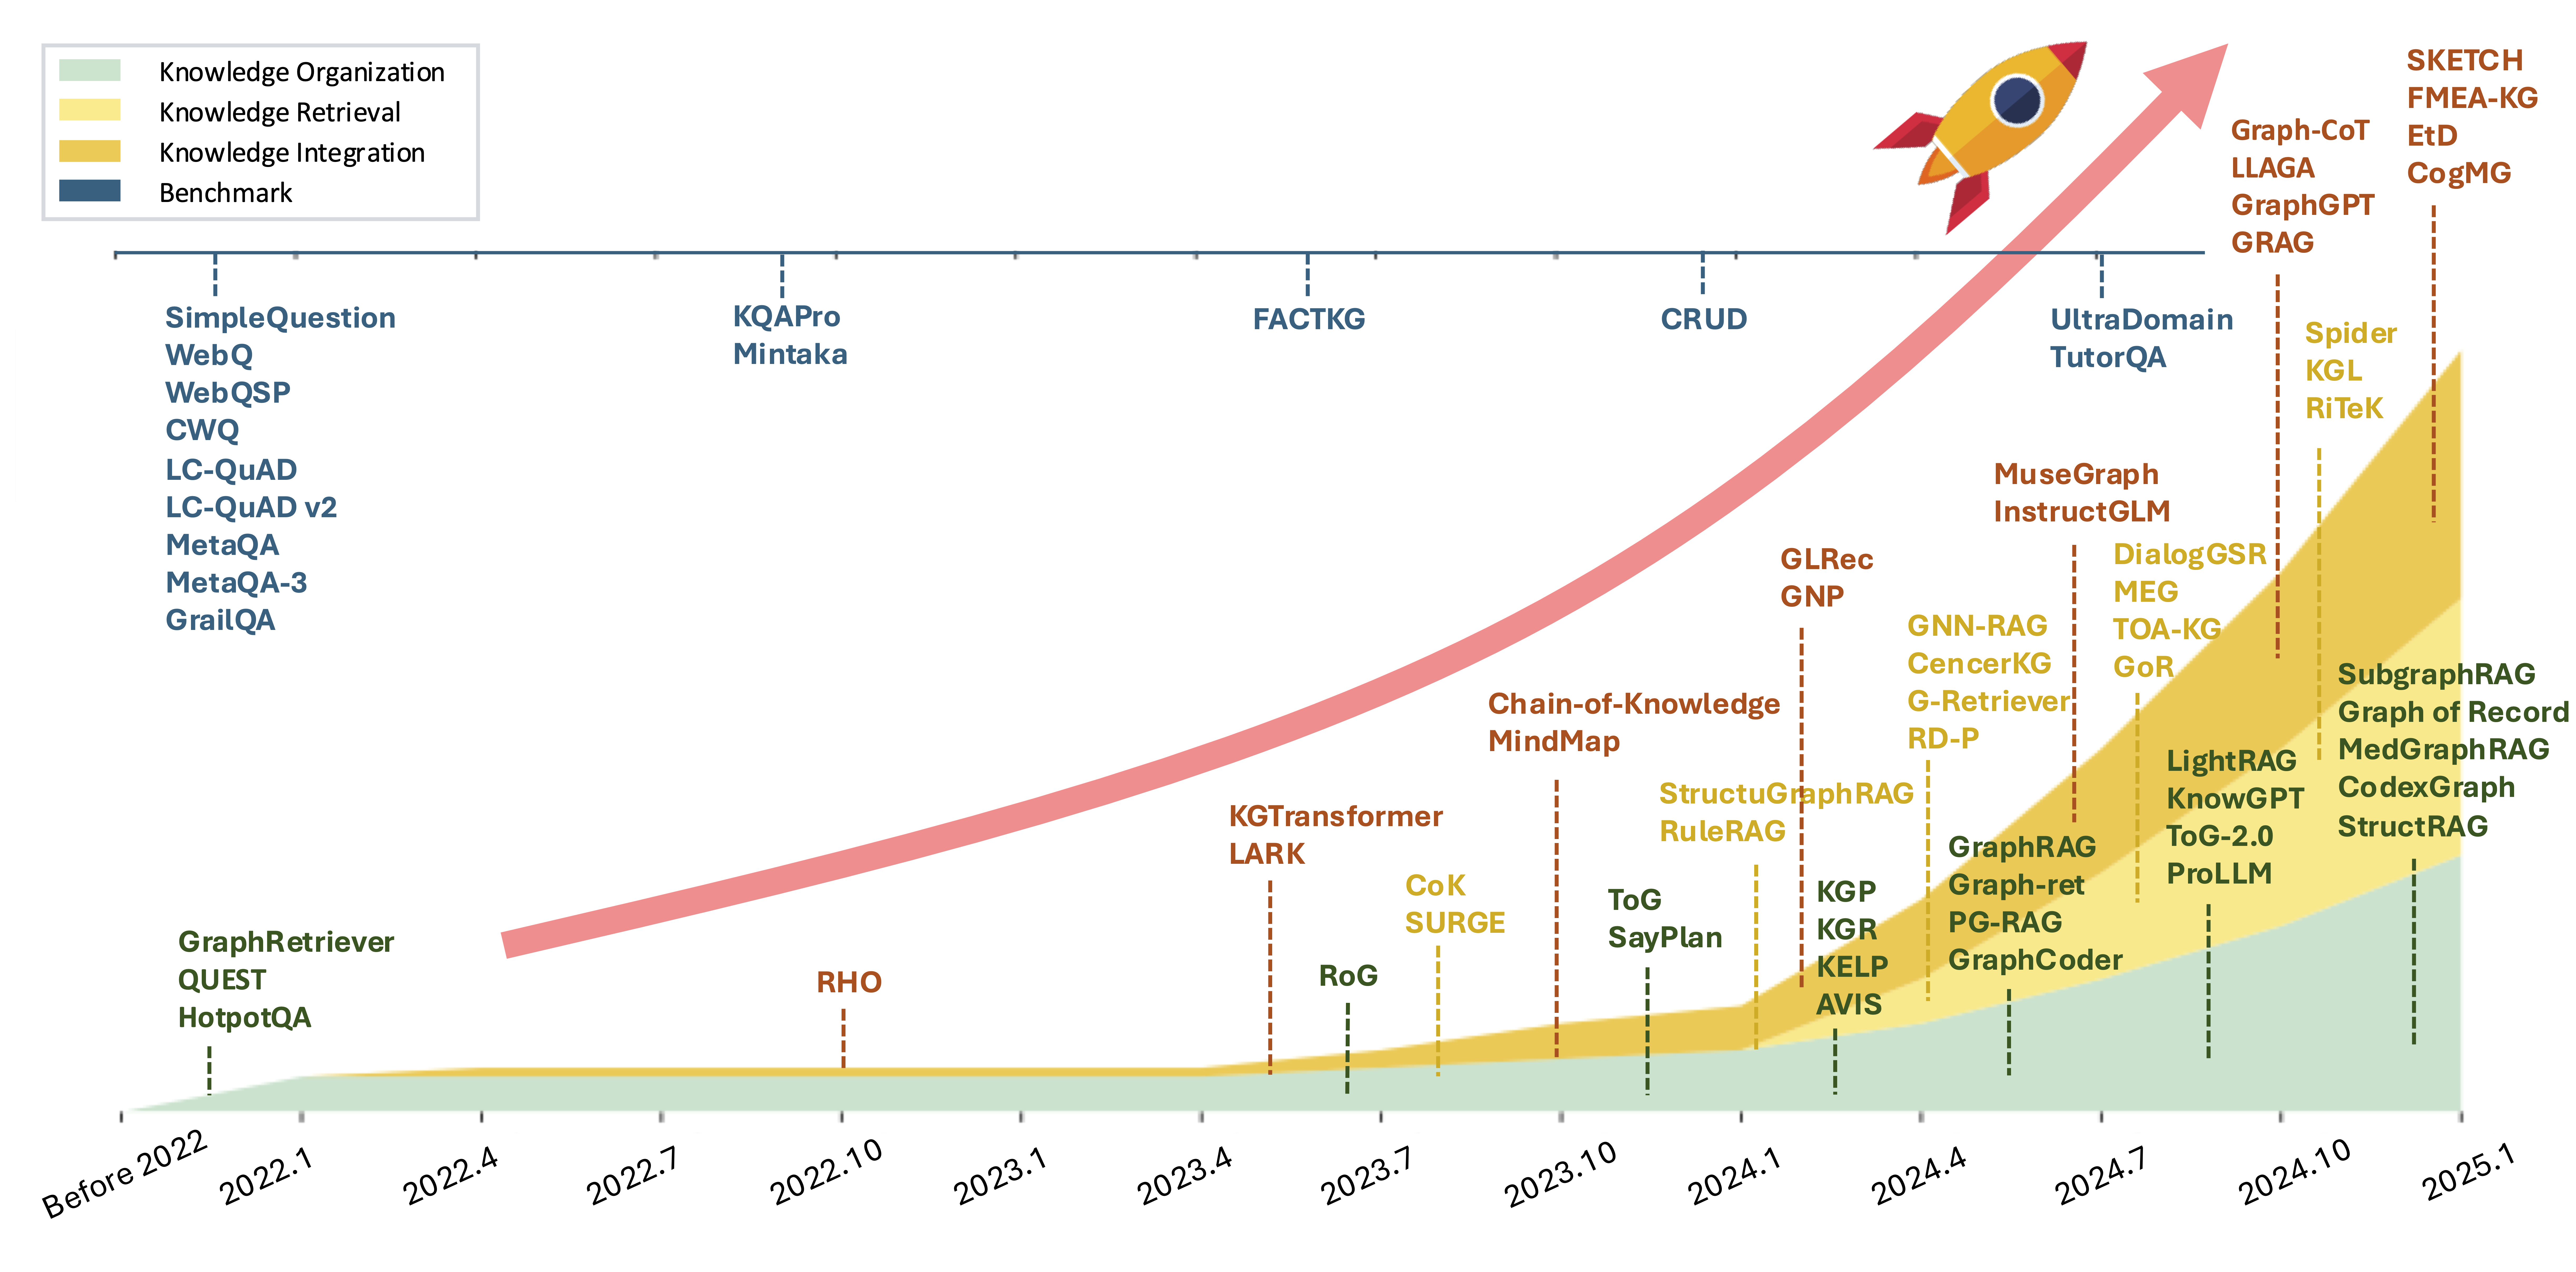
\includegraphics[width=\linewidth,keepaspectratio]{graphrag12}
	\end{center}
	
		{\tiny (Ref: Awesome-GraphRAG (GraphRAG Survey))}

	
\end{frame}

%%%%%%%%%%%%%%%%%%%%%%%%%%%%%%%%%%%%%%%%%%%%%%%%%%%%%%%%%%%
\begin{frame}[fragile]\frametitle{Conclusion}
    \begin{itemize}
        \item GraphRAG enhances traditional RAG models using structured knowledge.
        \item Improves accuracy, context-awareness, and efficiency.
        \item Useful in various domains like healthcare and banking.
        \item A promising approach for future AI-powered knowledge retrieval.
    \end{itemize}
\end{frame}


% %%%%%%%%%%%%%%%%%%%%%%%%%%%%%%%%%%%%%%%%%%%%%%%%%%%%%%%%%%%
% \begin{frame}[fragile]\frametitle{So, What is GraphRAG?}
    % \begin{itemize}
        % \item No universally accepted definition yet.
        % \item Some associate it with Microsoft's graph-based search approach.
        % \item Others define it as querying LPG or RDF graphs using LLM-generated queries (Cypher, SPARQL).	
        % \item Uses knowledge graphs instead of unstructured text.
        % \item Captures entities, relationships, and hierarchical structures.
        % \item Enables accurate, context-aware retrieval and response generation.
        % \item Supports complex query handling with enhanced explainability.
        % \item Combines structured Knowledge Graphs (KGs) with semantic vectors.
        % \item Enables LLMs to reason over multi-hop connections.
        % \item Provides a holistic perspective by connecting different data sources.		
    % \end{itemize}
% \end{frame}